\documentclass
[handout]
{beamer}
\documentclass{beamer}

%%
%%
%%
% From http://tex.stackexchange.com/questions/2072/beamer-navigation-circles-without-subsections
% Solution #2 or 3:
% \usepackage{etoolbox}
% \makeatletter
% % replace the subsection number test with a test that always returns true
% \patchcmd{\slideentry}{\ifnum#2>0}{\ifnum2>0}{}{\@error{unable to patch}}%
% \makeatother
% Solution #1:
\usepackage{remreset}% tiny package containing just the \@removefromreset command
\makeatletter
\@removefromreset{subsection}{section}
\makeatother
\setcounter{subsection}{1}


\usepackage{etex}
\usepackage{pgf}
\usepackage{tikz}
\usepackage{url}
\usepackage{amsmath}
\usepackage{color}
% \definecolor{red}{rgb}{1,0,0}
\usepackage{ulem}
% \usepackage{booktabs}
\usepackage{colortbl,booktabs}
\renewcommand*{\thefootnote}{\fnsymbol{footnote}}
\usepackage{fancybox}
\usepackage[framemethod=TikZ]{mdframed}
\mdfdefinestyle{FactStyle}{%
  outerlinewidth=0.5,
  roundcorner=1pt,
  leftmargin=1cm,
  linecolor=blue,
  outerlinecolor=blue!70!black,
  backgroundcolor=yellow!40
}
\usepackage{cancel}

  \newcommand\Warning{%
    \makebox[2.4em][c]{%
      \makebox[0pt][c]{\raisebox{.2em}{\Large!}}%
      \makebox[0pt][c]{\color{red}\Huge$\bigtriangleup$}}}%

\usepackage{stackengine}
\usepackage{scalerel}
\usepackage{xcolor}
  \newcommand\dangersign[1][2ex]{%
    \renewcommand\stacktype{L}%
    \scaleto{\stackon[1.3pt]{\color{red}$\triangle$}{\tiny !}}{#1}%
  }



\usepackage{dcolumn}
\newcolumntype{d}[1]{D{.}{.}{#1}}

% From
% http://tex.stackexchange.com/questions/109900/how-can-i-box-multiple-aligned-equations
\usepackage{empheq}
\usepackage{tcolorbox}  \newtcbox{\othermathbox}[1][]{%
  nobeforeafter, tcbox raise base, 
  colback=black!10, colframe=red!30, 
  left=1em, top=0.5em, right=1em, bottom=0.5em}

\newcommand\blue{\color{blue}}
\newcommand\red{\color{red}}
\newcommand\green{\color{green!75!black}}
\newcommand\purple{\color{purple}}
\newcommand\bluegreen{\color{blue!75!green}}
\newcommand\orange{\color{orange}}
\newcommand\redgreen{\color{red!50!green}}
\newcommand\grey{\color{black}}
\newcommand\gap{\vspace{.1in}}
\newcommand\nb{${\red\bullet}\ $}
\newcommand\halfgap{\vspace{.05in}}
\newcommand\divideline{\line(1,0){352}}
\usepackage{marvosym} % for \Smiley

\newcommand{\bluealert}[1]{{\blue\textbf{#1}}}

% \usepackage{beamerthemesplit} %Key package for beamer
\usetheme{Singapore}
% \usetheme{Szeged}
% \usetheme{Garfield}
% \usetheme{CambridgeUS}
% \usenavigationsymbolstemplate{} %Gets rid of slide navigation symbols


\setbeamercolor{separation line}{use=structure,bg=structure.fg!50!bg}
% \begin{beamercolorbox}[colsep=0.5pt]
%   {upper separation line foot}
% \end{beamercolorbox}



\makeatletter
\setbeamertemplate{footline}
{
  \leavevmode%
  \hbox{%
% \begin{beamercolorbox}[colsep=0.5pt]
%   {upper separation line foot}
% \end{beamercolorbox}


  \begin{beamercolorbox}[wd=.5\paperwidth,ht=2.25ex,dp=2ex,colsep=0.5pt]%
    {upper separation line foot}
    \usebeamerfont{author in head/foot}%
    \hspace*{2ex}\insertshortdate:\ \insertshorttitle
  \end{beamercolorbox}%
  \begin{beamercolorbox}[wd=.5\paperwidth,ht=2.25ex,dp=2ex,right]{title in head/foot}%
    \usebeamerfont{title in head/foot}
    {\insertshortauthor}\hspace*{2ex}
  \end{beamercolorbox}}%
  % \begin{beamercolorbox}[wd=.333333\paperwidth,ht=2.25ex,dp=2ex,right]{date in head/foot}%
  %   \usebeamerfont{date in head/foot}\insertshortdate{}\hspace*{2em}
  %   \insertframenumber{} / \inserttotalframenumber\hspace*{2ex} 
  % \end{beamercolorbox}%
  \vskip0pt%
}
\makeatother

\usetikzlibrary{decorations.markings}
\usetikzlibrary{arrows}


\title{Final Exam Review}
\author{Peter Garfield, UCSB Mathematics}
\date{March 15, 2017}
%\institute{}


\useinnertheme{default}

\usefonttheme{serif}
% \usecolortheme{rose}
% \usecolortheme{whale}
% \usecolortheme{orchid}
\usecolortheme{crane}
% \usecolortheme{dolphin}


%TEMPLATE
\setbeamertemplate{navigation symbols}{}

\setbeamertemplate{note page}[compress]

\setbeamertemplate{frametitle}{
  \vspace{0.5em}
  % \begin{centering}
  {\huge\blue\textbf{\textmd{\insertframetitle}}}
  \par
  % \end{centering}
}

% From http://tex.stackexchange.com/questions/7032/good-way-to-make-textcircled-numbers:
\newcommand*\circled[1]{\tikz[baseline=(char.base)]{\node[shape=circle,draw,fill=orange,inner sep=1pt] (char) {#1};}} 
% \renewcommand{\labelenumi}{\circled{\textbf{\arabic{enumi}}}}

\let\olddescription\description
\let\oldenddescription\enddescription
\usepackage{enumitem}
\let\description\olddescription
\let\enddescription\oldenddescription

% \usepackage[loadonly]{enumitem}
\setlist[enumerate,1]{label=\colorbox{orange}{\arabic*.},font=\bfseries}
%\setlist[enumerate,2]{label=\colorbox{blue!25}{(\alph*)},font=\bfseries}
% \setlist[enumerate,1]{label=\arabic*.,font=\bfseries}
\setlist[itemize,1]{label=\red$\bullet$}
\setlist[itemize,2]{label=\blue$\bullet$}

\newcommand\answer[1]{\fbox{#1}}
% \renewcommand\answer[1]{}

\newcommand{\antilog}{\operatorname{antilog}}








\title{}
\title{Calculus Intro}
\date{May 17, 2022}


\begin{document}
\small



\section*{Administration}

\frame{
  \frametitle{}
    {\Huge{}Welcome Back!}\\[.5em]

  {\Huge{}Differential Calculus}
  \vfill
  {\Large{}Instructor:}\\
  \ \hspace*{0.2in} \instructor
  
   \url{schley@math.ucsb.edu}\\
  \ \hspace*{0.2in} \officeloc
  \\[0.5em]

  {\Large{}Office Hours:}\\
  \ \hspace*{0.2in} \officehours 
  \bigskip

  \copyright\ 2022\ Daryl Cooper, Peter M.\ Garfield, Ebrahim Ebrahim \& Nathan Schley\\
  Please do not distribute outside of this course.
  \vfill

}



\section*{Review}


\frame{
Suppose $x$ and $y$ are related variables. So as one changes, the other changes.
We can ask:
\begin{center}
\textit{How much does $y$ change per unit change in $x$?}
\end{center}
Answer: The derivative of $y$ with respect to $x$ tells us, and it depends on the current value of $x$! 

\vspace{1em}

If we write $y$ as a function of $x$ like this: $y=f(x)$, then the derivative is written as
$$
\begin{array}{ccccc}
\dfrac{\textrm{d}y}{\textrm{d}x} & \text{or} & \dfrac{\textrm{d}f}{\textrm{d}x} & \text{or} & f'(x)
\end{array}
$$
It is the limit of ``average rate of change'' over shorter and shorter $\Delta x$:
$$ f'(x) = \lim_{h \rightarrow 0} \frac{f(x+h)-f(x)}{h} $$
also known as ``instantaneous rate of change''
}


\frame{
  \frametitle{Standard Estimation Problem}

  \alert{Question:}\ Approximate $\sqrt[3]{28}$.

  \begin{center}
    A$=0.111111$
    \quad 
    B$= 3.142857$
    \quad 
    C$ = 3.033333$
    \quad 
    D$ = 3.037037$
    \quad 
    E$ = 3.111111$
    \quad
    \uncover<3->{\fbox{D}}
  \end{center}

  \uncover<2->{%
    \alert{Hint:}\ If $g(x)=\sqrt[3]{x}$, then $g{\red'}({\blue 27})={\red
      1/27}$ and $g({\blue27}) = \sqrt[3]{\blue 27}={\bluegreen 3}$.
  }
  \gap
  \gap

  \uncover<4->{%
    \alert{Better estimate:}\ $\sqrt[3]{28}\approx3.036589$, so the {\red
      error} in the tangent line approximation here is
    \begin{equation*}
      \text{\red{}error} 
      \approx 3.037037-3.036589
      \approx.000448065
    \end{equation*}
    This is a percentage error of about $\red .015\%$.
  }

}


\frame{
  \frametitle{General Rule: (Review)}

  \begin{minipage}{0.45\linewidth}
    \begin{align*}
      \frac{d}{dx}\left(x^{\red 2}\right) & = {\red 2}x\\
      \frac{d}{dx}\left(x^{\red 3}\right) & = {\red 3}x^{\blue 2}\\
      \frac{d}{dx}\left(x^{\red 4}\right) & = {\red 4}x^{\blue 3}
    \end{align*}
  \end{minipage}
  \begin{minipage}{0.45\linewidth}
    \uncover<2->{%
      \begin{empheq}[box=\othermathbox]{align*}
        \frac{d}{dx}\left(x^{\red n}\right) & = {\red n}x^{\blue n-1}
      \end{empheq}
    }
  \end{minipage}
  \smallskip
  
  \uncover<3->{%
    The {\red exponent} comes out front. Then {\blue subtract} one
    from exponent.
  }

  \uncover<4->{\alert{Examples:}}
  \pause\pause\pause\pause

  \begin{enumerate}
  \item $\dfrac{d}{dx}\left( x^{\red 7}\right) = $
    \begin{center}
      A$ = 7x^7$
      \quad 
      B$ = 6x^6$
      \quad 
      C$ = 6x^7$
      \quad 
      D$ = 7x^6$
      \quad 
      E$ = 0$
      \quad
      \pause
      \answer{D}
    \end{center}

    \item $\dfrac{d}{dx}\left( x^{\red -3}\right) = $
      \begin{center}
        A$ = 3x^{-2}$
        \quad 
        B$ = -3x^{-2}$
        \quad 
        C$ = -2x^{-4}$
        \quad 
        D$ = -3x^{-4}$
        \quad
        \pause
        \answer{D}
      \end{center}

    \end{enumerate}

}


\frame{
  \frametitle{Why This Works (\S8.9)}
  \begin{empheq}[box=\othermathbox]{align*}
    \frac{d}{dx}\left(x^{\red n}\right) & = {\red n}x^{\blue n-1}
  \end{empheq}

  \uncover<2->{%
    \alert{Example: $n=3$:}\ Calculate the average rate of change of
    $x^3$ between ${\blue x}$ and $x+\text{{\red\only<3->{$h$}\only<2>{$\Delta
          x$}}}$ then take limit as
    {\red\only<3->{$h$}\only<2>{$\Delta x$}}$\to 0$.
  }

  \begin{align*}
    \uncover<4->{%
    \left(
    \begin{array}{c} 
      \text{average rate}\\ 
      \text{of change between}\\ 
      \text{$x$ and $x+{\red h}$}
    \end{array}
    \right)     
    }
    & \uncover<5->{ = \frac{({ {x}+{\red h}})^{3}-{ {x}^{ 3}}}{({x}+{\red h})-{ x}}}\\
    % & = \frac{({\green x}^3+3{\green x}^2{\purple h}+3{\green x}{\purple h}^2+{\purple h}^3)-{\blue {\green x}^3}}{{\purple h}}\\ 
    % \pause
    % & = \frac{3{\green x}^2{\purple h}+3{\green x}{\purple h}^2+{\red h}^3}{{\purple h}}\\ 
    % \pause
    & \uncover<6->{= 3x^2+3x{\red h}+{\red h}^2}
  \end{align*}
  \uncover<7->{%
    Limit as ${\red h}\to0$ is \colorbox{yellow}{$3x^2$}
  }
  \gap 
  
  \uncover<8->{%
    A similar calculation works for $x^{\red n}$ for any ${\red n}$.
  }
}





\frame{
  \frametitle{More Applications}

  \begin{enumerate}
    \setcounter{enumi}{2}
  \item  What is the equation of the tangent line at $x={1}$ to the 
    graph of  $y=x^3-x+4$?  The tangent line is $y=\ldots$? 
    \begin{center}
      A$ = x+3$
      \quad 
      B$ = 3x+1$
      \quad 
      C$ = 2x-2$
      \quad 
      D$=2x+2$
      \quad 
      E$=6x-2$
    \end{center}
  \end{enumerate}
  \uncover<2->{\alert{Answer:}\ \answer{D}}

  \uncover<3->{%
    Here's a picture:

    \begin{center}
      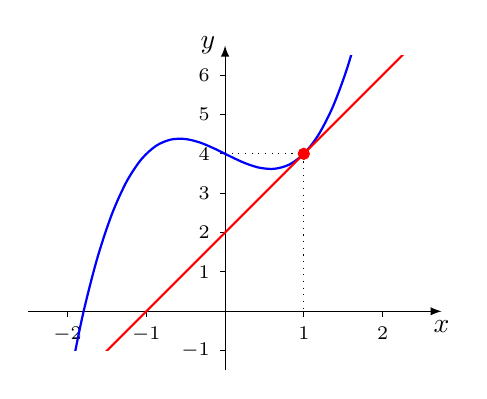
\begin{tikzpicture}[x=10mm,y=5mm,>=latex]
        \draw[thin,black,->] (-2.5,0) -- (2.75,0) node[below] {$x$};
        \draw[thin,black,->] (0,-1.5) -- (0,6.75) node[left] {$y$};
        % ticks:
        \foreach \x in {-2,-1,1,2}
        {
          \draw[thin,black] (\x,0) -- (\x,-2pt) node[below] {$\scriptstyle\x$};
        }
        \foreach \y in {-1,1,2,3,4,5,6}
        {
          \draw[thin,black] (0,\y) -- (-2pt,\y) node[left] {$\scriptstyle\y$};
        }
        \draw[thin,black,dotted] (0,4) -- (1,4) -- (1,0);
        \begin{scope}
          \clip (-2,-1) rectangle (2.5,6.5);
          \draw[thick,blue,domain=-2:2.5,smooth] plot (\x,{(\x)^3-\x+4});
        \end{scope}
        \begin{scope}
          \clip (-2,-1) rectangle (2.5,6.5);
          \draw[thick,red,domain=-2:2.5,smooth] plot (\x,{2*\x+2});
        \end{scope}
        \filldraw[red] (1,4) circle (2pt);
      \end{tikzpicture}
    \end{center}
  }
}

\frame{
  \frametitle{Another Example}

  \begin{enumerate}
    \setcounter{enumi}{3}
  \item The temperature in an oven after $t$ minutes is
    $50+t^3\ {}^{\circ}\,\text{F}$.  How quickly is the temperature
    rising after $2$ minutes?
    \begin{center}
      A$=58$
      \quad 
      B$ = 3$
      \quad 
      C$ = 12$
      \quad 
      D$ = 50$
      \quad 
      E$ = 8$
      \pause
    \end{center}
    \alert{Answer:}\ \answer{C}
  \end{enumerate}

}


\frame{
  \frametitle{Question}
We have a nice property of the derivative with addition, that 
$$\frac{d}{dx}(f(x) + g(x)) = f'(x) + g'(x).$$
\pause
For example, $x^3 + x^2$ has the derivative $3x^2 + 2x$.
\pause
How about multiplication? Is it true that 
$$\frac{d}{dx}\left(f(x)g(x)\right) {\red=} f'(x) \cdot g'(x)?$$
\pause
For example, $$\frac{d}{dx}(x\cdot x) {\red=} 1 \cdot 1?$$
\pause
\alert{\huge Nope!} 
\pause \\ 
$$\frac{d}{dx}(x\cdot x)=\frac{d}{dx}(x^2) = 2x$$




}


\frame{
     \frametitle{About Leibniz and the Product Rule}
``It is completely natural to wonder if the derivative of a product is given by that (false) rule. Nobody is saying Leibniz thought it might be true for any extended amount of time. According to p. 254 of ``The Historical Development of the Calculus" by C. H. Edwards, Leibniz wrote about his search for a product rule on November 11, 1675. He asked himself if $(uv)′=u′v$′ and quickly dismissed it by the example you gave: $u=v=x$. He did not know a correct product rule at the time. By July 11, 1677 he had the product and quotient rules (see p. 255 of the book by Edwards).'' \\ \\ 
-Keith Conrad


}


\frame{
  \frametitle{A Warning!}

  \begin{empheq}[box=\othermathbox]{align*}
    \ \hfill \raisebox{-0.5em}{\dangersign[6ex]} \hspace*{0.2in}
    \frac{d}{dx}\left(f(x)g(x)\right) {\red\ne} f'(x) \cdot g'(x)
    \hspace*{0.2in} \raisebox{-0.5em}{\dangersign[6ex]} \hfill \ 
  \end{empheq}
  \pause
  \bigskip

  \alert{Example:} \quad 
  $5x^4
  = \dfrac{d}{dx}\left(x^5\right)
  = \dfrac{d}{dx}\left(x^2\cdot x^3\right)
  {\red\ne}(2x)(3x^2)
  =6x^3$
  \bigskip
  \pause

  \alert{Example:} Find the derivative of $(x+1)(2x+3)$
  \bigskip
  \pause

  \alert{Question:}\ $\displaystyle\frac{d}{dx}\left((x^2+1)(x^3+1)\right)=$?
  \begin{center}
    A$=6x^3$
    \quad 
    B$ = 5x^4+3x^2+2x$
    \quad 
    C$ = x^5+x^3+x^2+1$
    \quad 
    D$ = \text{Other}$
  \end{center}
  \bigskip
  \pause

  \alert{Answer:}\ \fbox{B}

  \vspace*{2in}

}




\frame{
  \frametitle{Once upon a time\ldots} 

  There was a happy math professor and he told his
  happy students: 
  \medskip
  \pause

  ``When you work out {\blue derivatives} {\red ALWAYS} write the
  $\frac{d}{dx}$ part so you write something like
  \begin{empheq}[box=\othermathbox]{align*}
    \frac{d}{dx}\left(3x^2+5x+2\right) 
    & = 6x+5
  \end{empheq}
  and you never-ever-ever write\newline
  \begin{minipage}[b]{0.35\linewidth}
    \begin{empheq}[box=\othermathbox]{align*}
      3x^2+5x+2
      & \qquad 6x+5
    \end{empheq}
  \end{minipage}
  \hfill
  or even worse 
  \hfill
  \begin{minipage}[b]{0.35\linewidth}
    \begin{empheq}[box=\othermathbox]{align*}
      3x^2+5x+2
      =6x+5.
    \end{empheq}
  \end{minipage}
  \smallskip

  Because if you don't do as I say I will become a  sad   math professor and you will repeat this class.''

}


\frame{
  \frametitle{A Few Review Examples:}

  {\red(1)}\ If $f(x)=\sqrt{x}$, what is $f'(16)$?
  \begin{center}
    A$=\frac{1}{2}$
    \quad 
    B$=\frac{1}{4}$
    \quad 
    C$=\frac{1}{8}$
    \quad 
    D$=\frac{1}{16}$
    \quad 
    E$ = \frac{1}{32}$
    \pause
    \quad
    \fbox{C}
  \end{center}
  \bigskip

  {\red(2)}\ What is the $x$-coordinate of the point on the graph of
  $y=4x^2-3x+7$ where the graph has slope $13$? 
  \begin{center}
    A$=0$
    \quad 
    B$=1$
    \quad 
    C$=2$
    \quad 
    D$=3$
    \quad 
    E$=4$
    \pause
    \quad
    \fbox{C}
  \end{center}
  \bigskip

  {\red(3)}\ A circle is expanding so that after $R$ seconds it has
  radius $R$ cm.  What is the rate of increase of area inside the
  circle after $2$ seconds?
  \begin{center}
    A$=4\pi$
    \quad 
    B$ = 2\pi R^2$
    \quad 
    C$ =2$
    \quad 
    D$ = 2\pi R$
    \quad 
    E$ = \pi R^2$
    \pause
    \quad
    \fbox{A}
  \end{center}
  \bigskip

  % \gap $A(R)=$ area inside circle of radius $R$\\
  % {\red rate of increase of area
  %   = derivative}
  % = $\frac{d}{dR}\left(\pi R^2\right)=2\pi R$\hfill{\green explain}\pause\\
  % So rate of increase of area when $R=2$ is $2\pi(2)=4\pi$
  % 
  % \includegraphics[scale=0.5]{circlefirstordera.pdf}

}


\section{Exponential Functions}

\frame{
  \frametitle{Exponential Functions (\S8.8)}

  % {\blue(8.8) Exponential Functions} or why ${\red e^x}$ is {\red fun!}
  % \gap

  Is there a function $f(x)$ which equals its own derivative?  That
  is, can you find a function $f(x)$ with
  \begin{empheq}[box=\othermathbox]{align*}
    f'(x) & = f(x)?
  \end{empheq}
  \pause
  There are many many {\blue uses}\ for it.\pause
  \bigskip

  One boring answer: $f(x) = 0$.  Is there another?
  \pause
  \bigskip

  {\blue Yes}: 
  \begin{empheq}[box=\othermathbox]{align*}
    \frac{d}{dx} \big( e^x \big) & = e^{x}.
  \end{empheq}

  What's up with that?

}

\frame{
  \frametitle{The Derivative of $f(x) = a^x$}

  \begin{center}
    \begin{tikzpicture}[x=10mm,y=10mm,>=latex]
      \draw[thin,black,->] (-4.5,0) -- (4.5,0) node[below] {$x$};
      \draw[thin,black,->] (0,0) -- (0,5) node[left] {$y$};
      % Ticks:
      \foreach \x in {-4,-3,...,4}
      {
        \draw[thin,black] (\x,0) -- (\x,-2pt) node[below] {$\scriptstyle\x$};
      }
      \foreach \y in {1,2,3,4}
      {
        \draw[thin,black] (0,\y) -- (-2pt,\y) node[left] {$\scriptstyle\y$};
      }
      %
      \begin{scope}
        \clip (-4.5,0) rectangle (4.5,4.5);
        \uncover<2,11>{%
          \draw[thick,blue,domain=-4.5:4.5,smooth] plot (\x,{4^(\x)});
          \only<2>{\node[blue,right] at (1,4) {$y=4^x$};}
        }
        \uncover<3,11>{%
          \draw[thick,blue,domain=-4.5:4.5,smooth] plot (\x,{3^(\x)});
          \only<3>{\node[blue,right] at ({ln(4)/ln(3)},4) {$y=3^x$};}
        }
        \uncover<4,11>{%
          \draw[thick,blue,domain=-4.5:4.5,smooth] plot (\x,{2^(\x)});
          \only<4>{\node[blue,right] at (2,4) {$y=2^x$};}
        }
        \uncover<5,11>{%
          \draw[thick,blue,domain=-4.5:4.5,smooth] plot (\x,{(1.5)^(\x)});
          \only<5>{\node[blue,left] at ({ln(4)/ln(1.5)},4) {$y=1.5^x$};}
        }
        \uncover<6,11>{%
          \draw[thick,blue] (-4.5,1) -- (4.5,1);
          \only<6>{\node[blue,above] at (2,1) {$y=1^x = 1$};}
        }
        \uncover<7,11>{%
          \draw[thick,blue,domain=-4.5:4.5,smooth] plot (\x,{(1.5)^(-1*\x)});
          \only<7>{\node[blue,right] at ({-1*ln(4)/ln(1.5)},4) {$y=(2/3)^x$};}
        }
        \uncover<8,11>{%
          \draw[thick,blue,domain=-4.5:4.5,smooth] plot (\x,{2^(-\x)});
          \only<8>{\node[blue,left] at (-2,4) {$y=(1/2)^x$};}
        }
        \uncover<9,11>{%
          \draw[thick,blue,domain=-4.5:4.5,smooth] plot (\x,{3^(-\x)});
          \only<9>{\node[blue,left] at ({-1*ln(4)/ln(3)},4) {$y=(1/3)^x$};}
        }
        \uncover<10->{%
          \draw[thick,blue,domain=-4.5:4.5,smooth] plot (\x,{4^(-\x)});
          \only<10>{\node[blue,left] at (-1,4) {$y=(1/4)^x$};}
        }
      \end{scope}
      \uncover<11>{%
        \node[right,blue] at (4.5,1) {$1$};
        \node[above,blue] at ({ln(4.5)/ln(4)},4.5) {$4$};
        \node[above,blue] at ({ln(4.5)/ln(3)},4.5) {$3$};
        \node[above,blue] at ({ln(4.5)/ln(2)},4.5) {$2$};
        \node[above,blue] at ({ln(4.5)/ln(1.5)},4.5) {$1.5$};
        \node[above,blue] at ({-1*ln(4.5)/ln(1.5)},4.5) {$\frac{2}{3}$};
        \node[above,blue] at ({-1*ln(4.5)/ln(2)},4.5) {$\frac{1}{2}$};
        \node[above,blue] at ({-1*ln(4.5)/ln(3)},4.5) {$\frac{1}{3}$};
        \node[above,blue] at ({-1*ln(4.5)/ln(4)},4.5) {$\frac{1}{4}$};
      }
    \end{tikzpicture}
  \end{center}

  \uncover<11>{%
    \alert{Question:}\ Which ``$a$'' should we use?
  }
  \vspace*{1in}

}

\frame{
  \frametitle{The Derivative of $f(x) = a^x$}

  The slope of the graph at $x=0$ is 
  \begin{equation*}
    f'(0)
    = \lim_{h\to 0} \frac{ f(0+h) - f(0) }{h}
    = \lim_{h\to 0} \frac{a^h-a^0}{h}
    = \lim_{h\to 0} \frac{a^h-1}{h}
  \end{equation*}
  \pause

  This is a {\blue constant} that depends on what ${\red a}$ is.
  \pause

  Examples:
  \begin{equation*}
    \begin{array}{|l|c|c|c|c|c|}
      \hline
      \makebox[0.4in][l]{$a$} & \makebox[0.4in][c]{$1$} & \makebox[0.4in][c]{$2$} & \makebox[0.4in][c]{{\red$2.718\cdots$}} & \makebox[0.4in][c]{$3$} & \makebox[0.4in][c]{$4$} \\\hline
      f'(0) & $0$ & $0.6931$ & \makebox[0.4in][c]{{\red $1$}} & $1.0986$ & $1.3863$ \\\hline
    \end{array}
  \end{equation*}
  \pause
  \gap

  More generally,
  \begin{equation*}
    f'(x)
    \approx
    \frac{f(x+h)-f(x)}{h}
    \pause
    = \frac{a^{x+h}-a^{x}}{h}
    \pause 
    = \frac{a^{x}(a^h-1)}{h}
    \pause
    = a^{x} \left({ \frac{{a}^h-1}{h}}\right)
  \end{equation*}
  \pause

  \alert{Moral:}\ The derivative of $f(x) = a^x$ is a multiple of itself!
  \pause

  \alert{Second Moral:}\ That multiple is $1$ when $a =
  {\red2.718\,281\,828\cdots = e}$.
  % 2.718\,281\,828\,459\,045\cdots = e$.
}



\frame{
  \frametitle{Factorials}

  $5!=1\times 2\times 3\times 4\times 5$ is called {\red $5$
    factorial} and is the product of the whole numbers from $1$ up to
  $5$.  
  \smallskip

  What is $5!$?
  \begin{center}
    A$=5$
    \quad 
    B$ = 20$
    \quad 
    C$ = 60$
    \quad 
    D$ = 120$
    \quad 
    E$ = 720$
    \pause
    \quad
    \fbox{D}
  \end{center}
  \gap

  Why do we care? \pause
  There are $5!$ {\red{}orders}\ in which to trim the nails on your
  left hand. \pause 
  \gap

  Similarly $n!$ (``$n$ factorial'') is the product of all the whole
  numbers from 1 up to $n$.
  \gap

  \alert{Question:}\ What is $\dfrac{n!}{n}$?
  \begin{center}
    A$ = 1$
    \quad 
    B$ = n$
    \quad 
    C$ =  (n-1)!$
    \quad 
    D$ = (n+1)!$
    \pause
    \quad
    \fbox{C}
  \end{center}
  \gap

  Factorials come up a lot in {\blue probability and statistics}.

}

\frame{
  \frametitle{A Formula for $e^x$}

  It turns out that
  \begin{equation*}
    e^x 
    = 1+x+\frac{x^2}{2}+\frac{x^3}{6}+\frac{x^4}{24}+\frac{x^5}{120}+\cdots+\frac{x^n}{n!}+\cdots
  \end{equation*}

  How does it manage to equal it's own derivative? 


  \begin{align*}
    \uncover<2->{
    \frac{d}{dx}\left(e^x\right) 
    & = \frac{d}{dx}\left({\blue 1}+x+{\red\frac{x^2}{2!}}+{\green \frac{x^3}{3!}}+{\purple\frac{x^4}{4!}}+{\bluegreen \frac{x^5}{5!}}+\cdots\right)\\ 
    }
    & 
    \uncover<3->{%
      = {\blue 0}
    }
    \uncover<4->{%
      +1 
    }
    \uncover<5->{%
      +{\red\frac{2x}{2\times 1}}
    }
    \uncover<6->{%
      +{\green\frac{3x^2}{3\times2\times 1}}
    }
    \uncover<7->{%
      +{\purple\frac{4x^3}{4\times3\times 2\times 1}}
    }
    \uncover<8->{%
      +{\bluegreen \frac{5x^4}{5\times4\times3\times2\times1}} +\cdots\\
    }
    & \uncover<9->{%
      = {\blue 0}+1+{\red\frac{{\cancel{2}}x}{\cancel{2}\times 1}}+{\green\frac{\cancel{3}x^2}{\cancel{3}\times2\times 1}}+{\purple\frac{\cancel{4}x^3}{\cancel{4}\times3\times 2\times 1}}+{\bluegreen \frac{\cancel{5}x^4}{\cancel{5}\times4\times3\times2\times1}}+\cdots\\ 
    }
    & \uncover<10->{%
      = 1+{\red x}+{\green\frac{x^2}{2!}}+{\purple \frac{x^3}{3!}}+{\bluegreen \frac{x^4}{4!}}+\cdots\\ 
    }
    \uncover<11->{%
    & = e^x
      }
  \end{align*}

  \uncover<12->{%
    A simple {\red trick}: \parbox[t]{3in}{%
      \nb The derivative of each term is the preceding one. \\
      % \nb The derivative of the first term (which is the constant ${\blue 1}$) is zero.% {\red \Huge\Smiley}
      \nb The derivative of the first term is zero.% {\red \Huge\Smiley}
    }
  }

}


\frame{
  \frametitle{The Number $e$}

  The number $e={\blue2.718281828\cdots}$ is a very important in math.
  It can be calculated to as much accuracy as needed by using more and
  more terms in this formula for $e^x$ with $x=1$ plugged in:

  \begin{table}
    \begin{tabular}{|l||l|l|l|l|l|l|}\hline
      \text{$n$} & \raisebox{-1em}{\rule{0pt}{2.5em}}$\displaystyle1+1+\frac{1}{2}+\cdots +\frac{1}{n!} $\\
      \hline
      % 1 & 1  \\
      \hline
      1 & {\blue 2} \pause\\
      \hline
      2 & {\blue2}.5 \pause\\
      \hline
      3 & {\blue 2}.6666\ldots \pause\\
      \hline
      4 & {\blue 2.7}08333\ldots \pause\\
      \hline
      5 & {\blue 2.71}6666\ldots \pause\\
      \hline
      6 & {\blue 2.718}055\ldots \pause\\
      \hline
      7 & {\blue 2.7182}53968\ldots \pause\\
      \hline
      8 & {\blue 2.7182}78770\ldots \pause\\
      \hline
      9 & {\blue2.718281}526\ldots \pause\\
      \hline
      10 & {\blue 2.7182818}01\ldots \pause\\
      \hline
      {\blue  exact} & {\blue 2.7182818284590452354...}\\
      \hline
    \end{tabular}
  \end{table}

  % You must remember {\red this} \pause $\cdots$\pause  \fbox{\red $e^0=1$}


}

\frame{
  \frametitle{Key Facts about $e$ and $e^x$}
  
  What you need to remember:
  \begin{itemize}
  \item[\nb] $e^0  = 1$
    \smallskip

  \item[\nb] $\dfrac{d}{dx} \big( e^x \big)  = e^x$
    \bigskip
  \end{itemize}
  \pause
  
  \alert{Question:}\ What is the equation of the tangent line to
  $y=e^x$ at $x=0$?
  \begin{center}
    A $y = 1$
    \quad 
    B $y = x$
    \quad 
    C $y = x+1$
    \quad 
    D $y = ex+1$
    \pause
    \quad\fbox{C}
  \end{center}

  \begin{center}
    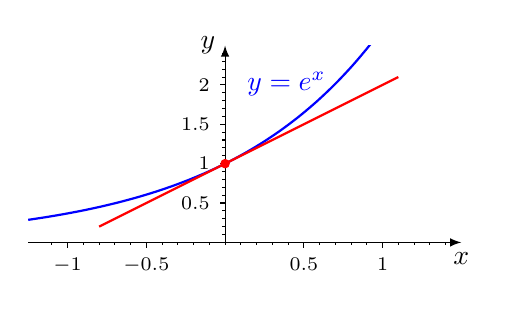
\begin{tikzpicture}[x=20mm,y=10mm,>=latex]
      \draw[thin,black,->] (-1.25,0) -- (1.5,0) node[below] {$x$};
      \draw[thin,black,->] (0,0) -- (0,2.5) node[left] {$y$};
      % Ticks:
      \foreach \x in {-1.1,-1,...,1.42}
      {
        \draw[thin,black] (\x,0) -- (\x,-1pt);
      }
      \foreach \x in {-1,-0.5,0.5,1}
      {
        \draw[thin,black] (\x,0) -- (\x,-2pt) node[below] {$\scriptstyle\x$};
      }
      \foreach \y in {0.1,0.2,...,2.43}
      {
        \draw[thin,black] (0,\y) -- (-1pt,\y);
      }
      \foreach \y in {0.5,1,1.5,2}
      {
        \draw[thin,black] (0,\y) -- (-2pt,\y) node[left] {$\scriptstyle\y$};
      }
      %
      \begin{scope}
        \clip (-1.25,0) rectangle (1.5,2.5);
        \draw[thick,blue,domain=-1.25:1.5,smooth] plot (\x,{exp(\x)});
        \node[blue,left] at (0.7,{exp(0.7)}) {$y=e^x$};
        \draw[thick,red,domain=-0.8:1.1,smooth] plot (\x,{1+\x});
      \end{scope}
      \filldraw[red] (0,1) circle (1.5pt);
    \end{tikzpicture}
  \end{center}

}

\section{Differentiating $e^{kx}$}
\frame{
  \frametitle{Differentiating $f(x) = e^{kx}$}

  \begin{minipage}[b]{0.35\linewidth}
    \begin{empheq}[box=\othermathbox]{align*}
      \frac{d}{dx}\left(e^{{\red k}x}\right) 
      & = {\red k}e^{{\red k}x}
    \end{empheq}
  \end{minipage}
  \hspace*{0.2in} \pause
  versus
  \hspace*{0.2in}
  \begin{minipage}[b]{0.35\linewidth}
    \begin{empheq}[box=\othermathbox]{align*}
      \frac{d}{dx}\left(x^{{\red n}}\right) 
      & = {\red n} x^{{\red n}-1}
    \end{empheq}
  \end{minipage}
  \bigskip
  \pause \\
These are different functions. \pause Both use exponents, sure, but in very different ways! \pause
  \begin{empheq}[box=\othermathbox]{align*}
    \raisebox{-0.5em}{\dangersign[6ex]}  
    \hspace*{0.1in}
    \text{Be careful not to write}\ 
    \dfrac{d}{dx} \big( e^{{\red k}x} \big) = {\red k}e^{({\red k}-1)x}.
    \hspace*{0.1in}
    \raisebox{-0.5em}{\dangersign[6ex]}  
  \end{empheq}
  \bigskip
  \pause

  \alert{Question:}\ Find $\dfrac{d}{dx}\left( 4e^{3x}+ 5x^3\right)$
  \begin{center}
    A$=12e^{2x}+15x^2$
    \qquad 
    B$ = 12e^{3x}+15 x^3$
    \qquad 
    C$ = 4e^{3x}+15x^2$
    \\
    \ 
    \quad 
    D$=12e^{3x}+15x^2$
    \quad
    E$= \text{Other}$
    \pause
    \quad
    \fbox{D}
  \end{center}

}

















\end{document}


